\documentclass[12pt, twocolumn]{article}
\usepackage[utf8]{inputenc}
\usepackage{amsmath}
\usepackage[margin = 1.1in]{geometry}
\usepackage{float}
\usepackage{graphicx}
\graphicspath{{images/}}
\setlength{\columnsep}{0.75cm}
\usepackage{hyperref}
\usepackage{tfrupee}
\hypersetup{
colorlinks=true,
    linkcolor= red,
    }

\title{AI1110 Assignment 1}
\author{MALOTHU AVINASH AI21BTECH11018}
\date{March 2022}

\begin{document}
\maketitle
\textbf{Q5(B):} Rekha opened a recurring deposit account for 20 months. The rate of interest is 9\% per annum and Rekha receives \rupee441 as interest at the time of maturity.
Find the amount Rekha deposited each month.
\\\textbf{Solution:}\\
According to given question
\\Rekha opened a recurring deposit account for 20 months(n),
\\Rate of interest(r) is 9\% per annum,and Rekha receives \rupee 441 as interest at the time of maturity.

{\\$$ From\;simple\;interest\;formula\;I=p\cdot\ t\cdot\frac{r}{100}
\\
\\
$$Total\;Interest(i) = x\cdot\frac{1}{12}\cdot\frac{9}{100} + x\cdot\frac{2}{12}\cdot\frac{9}{100} + x\cdot\frac{3}{12}\cdot\frac{9}{100} +
---- +x\cdot\frac{20}{12}\cdot\frac{9}{100}$$
\\
\\ $$Given\;Total\;Interest \; is \; 441 \; then$$
\\
\\$$441 = x\cdot\frac{9}{1200}(1+2+3+----+20)$$
\\
\\ $$x = \frac{441\cdot1200\cdot2}{9\cdot20\cdot21}$$
\\
\\$$ Finally\;we\;get \; x = 280 \\\;c\;code\;output\;as\;follows
\\ }
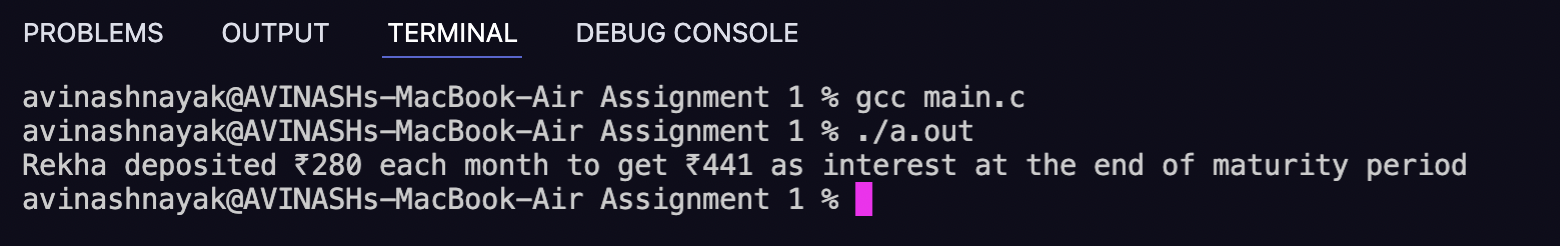
\includegraphics[width=\textwidth]{solution.png}

\end{document}
